\section{Дальнейшее развитие алгебры}
После инновационной Алгебры Аль-Хорезми, развитие алгебры не остановилось. Несколько мусульманских математиков известны своми работами в области алгебры.

\subsection{Сабит ибн Курра}
Сабит ибн Курра (836-901 н.э.) продолжил общие решения Аль-Хорезми; однако Аль-Хорезми представляет свои общие доказательства в
соединение с конкретными уравнениями, тогда как ибн Курра представляет свои решения обобщенно. В свое время ибн Курра имел полный доступ к Началам Евклида и свободно использовал теоремы Евклида в своих алгебраических доказательствах. 

В случае $x^2 + px = q$, Сабит ибн Курра верно находит, что $x = \sqrt{q + (\frac{p}{2})^2} - (\frac{p}{2})$. Он приводит общие доказательства, следуя примерам <<определение - теорема - доказательство>> Евклида.

\subsection{Абу Камил}
Абу Камил (около 850-930 н.э.) написал трактат под названием «Алгебра», который был комментарием к работе Аль-Хорезми. Его примеры позже были использованы как мусульманским ученым Аль-Караджи в конце 10 века, так и итальянским Леонардо Пизанским или Фибоначчи в конце 12 века. Многие из его примеров взяты из Аль-Хорезми. Абу Камиль также рассматривает геометрические доказательства решений уравнений в терминах конкретных примеров, как Аль-Хорезми, вместо использования общих доказательств, таких как Сабит ибн Курра. Абу Камиль выходит за пределы алгебры Аль-Хорезми и Сабит ибн Курра, предоставляя правила манипулирования следующими алгебраическими величинами:

$$(a \pm b)(b \pm qx) = ab \pm bpx \pm aqx + pqx^2$$
$$(a \pm b)(b \mp qx) = ab \pm bpx \mp aqx - pqx^2$$
$$\sqrt{ab} = \sqrt{a}\sqrt{b}$$
$$\sqrt{a/b} = \sqrt{a}/\sqrt{b}$$
$$\sqrt{a} \pm \sqrt{b} = \sqrt{a + b \pm 2\sqrt{ab}}$$

Абу Камиль дает как алгебраические, так и геометрические доказательства для этих уравнений.

\subsection{Абу Бакр Аль-Караджи}
Аль-Караджи (953-1029 н.э.) имеет тенденцию применять арифметику к алгебре, в отличие от Абу Камиля и Ибн Курры, которые применяют геометрию к алгебре. Абу Бакр Аль-Караджи написал \textit{Дивный}, в котором он развивает алгебру выражений с использованием высших степеней неизвестного. Он использует «корень», «сторону» или «вещь» для обозначения x, «mal» для x2, «куб» для x3, «mal mal» для x4, «mal куб» для x5 и т. д. Он создает каждую степень неизвестного путем умножения на предыдущие элементы; это новшество позволило аль-Караджи обращаться с такими уравнениями, как $x^4 + 4x^3 - 6$ и $5x^6 - (2x^2 + 3)$

\subsection{Аль Самуил (Самуил Марокканский)}
Ибн Яхья Аль-Магриби Аль-Самуил (1130-1180 гг. Н. Э.) Родился в Багдаде. Хотя он родился в еврейской семье, он обратился в ислам в 1163 году, когда ему приснился сон, говорящий ему об этом. Он был известным врачом и путешествовал по современному Ирану, чтобы заботиться о своих пациентах, в том числе о принцах. Его «Сияющая книга расчетов» дает правила для знаков, создавая понятия положительных (избыточных) и отрицательных (дефицитных) чисел. Затем он дает правила вычитания степеней:

$$(-ax^n) - (-bx^n) = -(ax^n - bx^n) \textrm{ ,если } a > b$$
$$(-ax^n) - (-bx^n) = +(bx^n - ax^n) \textrm{ ,если } a < b$$

Аль-Самуил излагает диаграмму, чтобы научить читателя, как умножать и делить
простые выражения, такие как «часть mal куба» или «mal mal куб, который
равны $\frac{1}{x^5}$ и $x^7$

Он также приводит примеры деления сложных многочленов, что было большим развитием в алгебре. Его первый пример показывает, как решить:

$$\frac{20x^6 + 2x^5 +58x^4 + 75x^3 + 125x^2 + 96x + 94 + 140x^-1 + 50x^-2 + 90x^-3 + 20x^-4}{2x^3 + 5x + 5 + 10x^-1}$$

Он создает диаграмму (рисунок ниже) с верхней строкой как имена порядков в естественной последовательности слева направо, а строка ниже - как строка ответа, которая начинается пустой и заполняется по мере продолжения. Остальная часть диаграммы разделена на горизонтальные полосы с двумя рядами каждая:

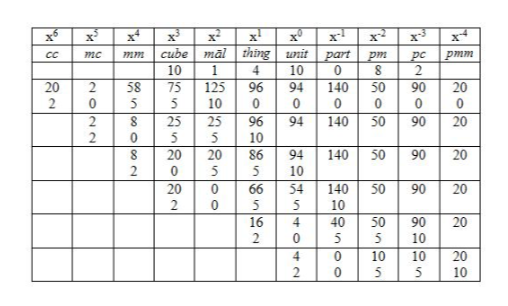
\includegraphics[scale=0.7, center]{4}

Аль-Самуил начинает с деления $20cc$ на $2c$ для получения $10c$, а затем вычитает ($10c \times$ делитель) из делимого. Старое делимое заменяется остатком после вычитания, а делитель копируется вправо. Повторяя эту процедуру, 2 нового делимого делится на 2 делителя, а частное 1 помещается в столбец справа от 10 в строке ответа. Аль-Самуил продолжает повторять процедуру до тех пор, пока не достигнет своего конечного результата:

$$10x^3 + x^2 + 4x + 10 + 8x^-2 +2x^-3$$

Аль-Самуил следует этому примеру с несколькими другими, повторяя ту же процедуру, но допуская отрицательные коэффициенты. Его открытие процедуры деления в столбик было значительным достижением в исламской алгебре.

\subsection{Омар Хайям}
Полное имя Омара Хайяма - Абу аль-Фат Омар бен Ибрагим Аль-Хайям и родился в современном Иране. Дословный перевод его имени означает «делатель палаток». Это, возможно было дело его отца. Хайям стал известен в результате популярного перевода Эдварда Фитцджеральда в 1859 году почти 600 коротких четырех стихотворений - Рубайята.

Его блестящий вклад был продолжен в XIX веке. Среди многих других он работал над вопросами, связанными c постулатом о параллельным прямых (пятый постулат Евклида). Используя четырехугольник, он обнаружил подход к исследованию, став стандартным. Он точно обнаружил, что нужно показать, чтобы доказать постулат о параллельных прямых, и именно на этих идеях была обнаружена неевклидова геометрия. Хайям также утверждал, что рациональные числа должны охватываться цифрами, отступающими от греческой традиции, влияние которых было тогда и должно было оставаться мощной силой в математике и философии до XIX века.

Он также обнаружил методы извлечения корня в сколь угодно большой степени. Он обнаружил (в алгебре) геометрический метод решения кубических уравнений путем пересечения параболы с кругом, но, по крайней мере частично, эти методы были описаны более ранними авторами, такими как Абу аль-Джуд. Чтобы увидеть, рассмотрим круг и параболу:

$$(x - a)^2 + y^2 = a^2 + c^2, y = x^2 + bx + c$$

Заменим и упросим:
$$x(x^3 - 2bx^2 -x -2cx -xb^2 +2a -2cb)$$

Что даст при делении:
$$x(x^3 + 2bx^2 +(1 + 2c + b^2)x + 2cb - 2a) = 0$$

Итак, пересечение x является решением кубического уравнения:

$$x^3 + 2bx^2 + (1 + 2c + b^2)x + 2cb - 2a$$
Хайям был выдающимся математиком и астрономом. Его работа над алгеброй была известна во всей Европе в средние века, и он также внес вклад в календарную реформу. Хайям упоминает в своей книге Алгебры другую работу, которая теперь потеряна. В этой потерянной работе Хайям обсуждает треугольник Паскаля, но китайцы, возможно, обсуждали треугольник перед этой датой.

Алгебра Хайяма является геометрической, решая линейные и квадратичные уравнения методами, появляющимися в Началах Евклида.

Известность Хайяма как поэта заставила некоторых забыть о его научных достижениях, которые были гораздо более существенными. Версии форм и стихов, используемых в Рубайяте, существовали в персидской литературе до Хайяма, и немногие из его стихов можно было отнести к нему с уверенностью.
